\documentclass{article}
\usepackage{amsthm}
\usepackage{amsmath}
\usepackage{mathtools}
\usepackage{amssymb}
\usepackage{chngcntr}
\usepackage[margin=1.2in]{geometry}
\usepackage{graphicx}
\usepackage{caption}
\usepackage{hyperref}
\usepackage{graphicx}
\graphicspath{ {images/} }

\counterwithin*{equation}{section}
\counterwithin*{equation}{subsection}

\title{Semantic Analyzer for COOL}
\author{Ganesh Vernekar - CS15BTECH11018 \\ Sukrut Rao - CS15BTECH11036}


\begin{document}
	\maketitle
	
This assignment creates a Semantic Analyzer for the COOL language. The output for a correct input program is a type annotated abstract syntax tree. The program performs semantic checks and reports errors for incorrect programs. All COOL rules are taken into account except that it is assumed that there is no \verb|SELF_TYPE|.
	
\section{Code Design}
\subsection{Overview}
At a high level, the program does the following steps:
\begin{enumerate}
	\item Traverse the input program and prepare an inheritance tree of all the classes. Checks are in place to ensure that there is no cycle in this directed tree. A check is also made to ensure that the class \verb|Main| exists.
	\item Prepare a map of each function with its mangled name with the class name (called the \textit{Cl-mangled name}) with the function's return type. The name of the function is mangled to hold its name, list of arguments with types, and the class name, but not the return type. This is mapped against its return type, with the purpose of checking if dispatches made from other classes' objects in a given class are valid.
	\item Traverse the AST in using the visitor pattern. At each node, scopes are entered and exited as applicable, and lookups are performed appropriately. Type annotations are done for each node after completing it for all of its children. Two scope tables are used - one for attributes and parameters, and the other for functions. The scope table for functions maps each function to its mangled name with return type, called the \textit{RT-mangled name}.
\end{enumerate}
At each stage, errors are reported as they are found, and attempts to recovery are made. The output of a semantically correct program is a type annotated AST, and that of a semantically incorrect program is a set of error messages.

\subsection{Preparing the inheritance graph}
This is the first pass on the input program, which is in the form of the AST. The program starts by visiting the root of the AST. This pass takes place while visiting the root, in \verb|VisitorImpl.java|, before it continues its traversal down the AST. The following steps take place:
\begin{enumerate}
	\item An inheritance graph, an object of the class \verb|InheritanceGraph| defined in \verb|InheritanceGraph.java| is created. This also defines a type, \verb|Node|, to represent each node in the graph.
	\item During the creation, all the base classes, that is, \verb|Object|, \verb|IO|, and \verb|String|, are added to the graph, with \verb|Object| as the root. \verb|Int| and \verb|Bool| are not directly added as a node, they are only added to a hash map containing the indices of the nodes of each class in the graph, with a dummy index of $-1$. This is done for convenience as neither of these classes define any methods, nor can they be inherited from, and thus serve as a special case.
	\item The graph is stored as an \verb|ArrayList| of nodes. The indices of each node are stored in a hash map, that maps the name of the class to its index. This helps in quick lookup of a node from the class name, and helps check if the class exists in the graph or not.
	\item In \verb|VisitorImpl.java|, from the \verb|program| node, each class is iterated over and added to the inheritance graph. A check is made to ensure that a class is not redefined, and hence not added twice. If a class is redefined, an error is reported and the redefinition is not added to the graph.
	\item Then, the graph is analyzed to check for the presence of directed cycles in the graph. Here, the presence of the \verb|Main| class is also checked. If there is either a cycle or no \verb|Main| class, errors are reported and the compilation terminates. If not, the inheritance graph is ready.
\end{enumerate}
At the end of this pass, if there are no errors, it can be asserted that the inheritance graph is valid, and that there exists a \verb|Main| class. 

\subsection{Populating the Cl-mangled name}
Once the inheritance graph is ready, the program next prepares a map of the \textit{Cl-mangled name} of each function with its return type.
\subsubsection*{Definition of the Cl-mangled name}
The Cl-mangled name of a method is a name that contains the method name, its argument list along with their types, and the name of the class it belongs to. The return type is not a part of the Cl-mangled name.\\
The following is the procedure to construct this name. Suppose we have a method \\ \verb|func(x : Int, y : String) : Bool| defined in class \verb|Cl|:
\begin{enumerate}
	\item The mangled name starts with \verb|_CN|, followed by the number of characters in the class name, followed by the name. In our case, it will be \verb|_CN2Cl|.
	\item Then, it is appended with \verb|_FN|, followed by the number of characters in the method name, and then the name. In our example, we now have \verb|_CN2Cl_FN4func|.
	\item This is followed by \verb|_AN|, where \verb|A| stands for argument, followed by the number of parameters in the function, followed by \verb|_|. Here, we have \verb|_CN2Cl_FN4func_AN2_|.
	\item A counter starting from $0$ is appended to mark the argument number. Then, \verb|N| is appended, followed by the length of the argument type name, followed by the argument type name. We now have \verb|_CN2Cl_FN4func_AN2_0N3Int1N6String|.
	\item The name where there are non-zero parameters, ends with \verb|_FT_|, to stand for "formal true". The complete mangled name thus is \verb|_CN2Cl_FN4func_AN2_0N3Int1N6String_FT_|.
	\item If there were no parameters, it ends with \verb|_FF_|. The name in our case would then have been \verb|_CN2Cl_FN4func_AN0__FF_|.
\end{enumerate}
	
\subsubsection*{Purpose and usage of the Cl-mangled name}
A mangled name map is created that maps the Cl-mangled name of each function with its return type. In the example above, the name  \verb|_CN2Cl_FN4func_AN2_0N3Int1N6String_FT_| would be mapped with \verb|Bool|. This is done by traversing across each class node from the program node and then traversing across each feature node for each class node. The purpose of this is to easily perform type checking for dispatches, especially for objects of other classes. In a class \verb|A|, suppose a dispatch is performed of \verb|func()| from class \verb|Cl|. The program needs to check if the dispatch parameters are of valid types, and if the object it is called on has a valid type. While traversing the AST, we might have not yet reached the class \verb|Cl|, and hence the method would not be type annotated yet. So, this provided an easy solution to perform the validity check quickly without leaving the current AST node.

~\\
At the end of this pass, the Cl-mangled names of each method in the input program have been mapped to their return types.

\subsection{Parsing inheritance graph by maintaining scope data}

A depth first traversal is done which prevents multiple time repopulation of scope data of a class. We explain this with an example below.
\begin{itemize}
	\item Here a single node refers to a class in the program.
	\item The graph is an inheritance graph. \verb|B inherits A|, \verb|D inherits B|, and so on.
	\item \verb|Yellow| nodes are the ones which is being currently visited.
	\item \verb|Blue| nodes are the ones whose data is currently in the scope.
	\item \verb|Green| nodes are the ones which has already been visited.
\end{itemize}

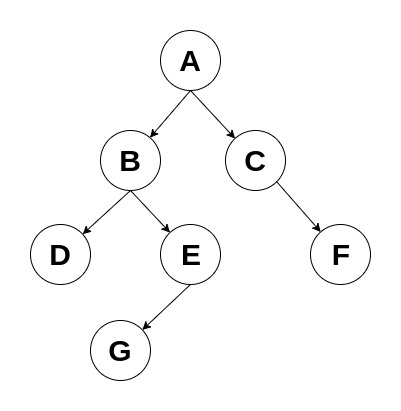
\includegraphics[width=3cm]{1.jpg}
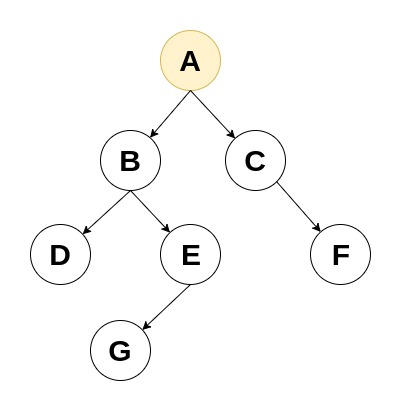
\includegraphics[width=3cm]{2.jpg}
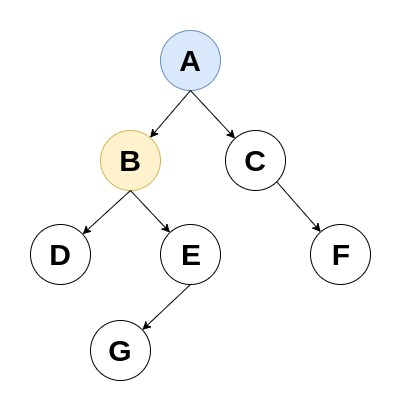
\includegraphics[width=3cm]{3.jpg}
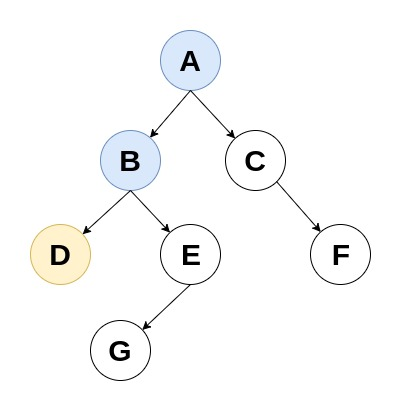
\includegraphics[width=3cm]{4.jpg}
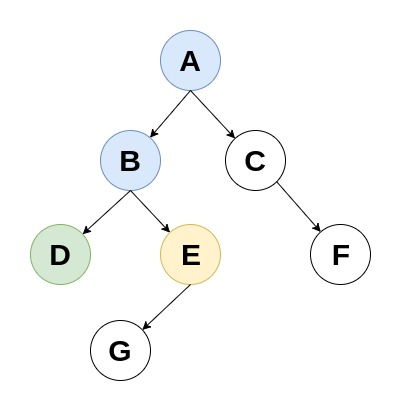
\includegraphics[width=3cm]{5.jpg}
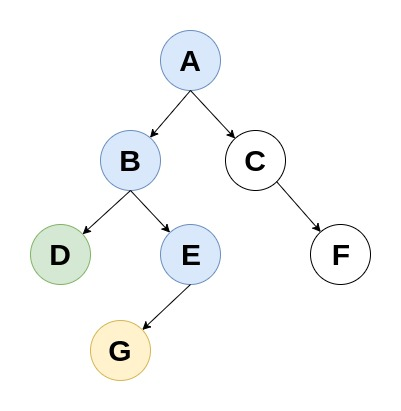
\includegraphics[width=3cm]{6.jpg}
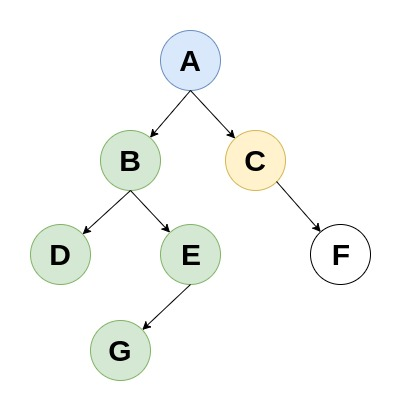
\includegraphics[width=3cm]{7.jpg}
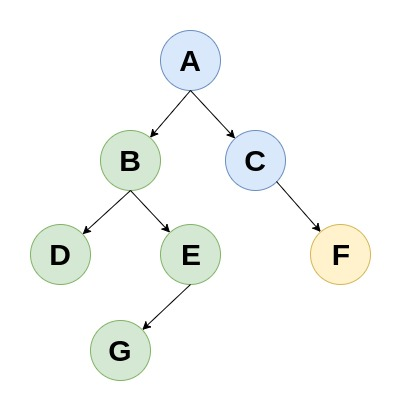
\includegraphics[width=3cm]{8.jpg}
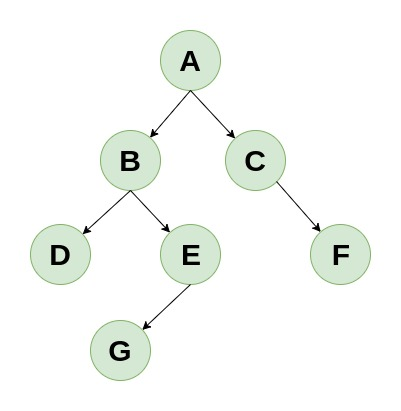
\includegraphics[width=3cm]{9.jpg}

~\\
We start the parsing process from the root. When we are visiting a node, we enter next level of scope and store all its data in that scope. After visiting that node, we retain the scope data and go ahead to visit its children. Once all the children are visited (recursively), we discard the data of this scope by exiting the scope and move above the tree.

~\\
In this way we enter a new scope for a node only once while the children of a node still get the data from the parents.

\subsection{Handling Scope}\label{handlingscope:f}
This section describes how scope checking is handled by the program. The program consists of two scope tables :
\begin{enumerate}
	\item V-Scope table
	\item F-Scope table
\end{enumerate}

\subsubsection*{V-Scope table}
This is the scope table in the usual sense, that stores each identifier and its type. The implementation is the pre-defined implementation given in this assignment. When the program enters a new scope of the input program, a new scope of the scope table, in the form of a new hash map is entered. When the program exits a scope of the input program, the scope is exited. At any given point, only the scopes from the current scope to a chain of directly outer scopes is stored. For example, if a class \verb|Cl| has methods \verb|f1()| and \verb|f2()|, and \verb|f1()| is visited first, its scope is destroyed when the program reaches \verb|f2()|.
\\
This works because attributes of another class object cannot be accessed directly, and hence, their scopes need not be stored. Methods can be accessed directly using a dispatch, and to handle this, we already have the map containing the Cl-mangled name.
\\
Thus, for any legal usage of an identifier, it must lie in the current scope or any scope in the chain of outer scopes. For methods, the scope checking is handled using the map of Cl-mangled names. Hence, this saves memory and keeps the structure of the table simple.

\subsubsection*{F-Scope table}
This is another scope table, that maps the method name with its \textit{RT-mangled name}. This mangled name form contains the method name, its number and types of arguments, and its return type. The class name is not a part of the RT-mangled name, while the return type is, unlike the Cl-mangled name.
\\
The purpose of this is to check for definitions of methods with the same name in a class and its ancestors. The benefit is four-fold:
\begin{enumerate}
	\item Checks that multiple methods with the same name do not exist in the same class.
	\item Checks whether a call to a method not defined in the current class is defined in an ancestor class.
	\item Checks that a function redefined from an ancestor class has the same signature and the same return type.
	\item Checks that the \verb|main()| method exists in the \verb|Main| class.
\end{enumerate}
This is a separate scope table as it would be possible to have an identifier with the same name as the RT-mangled name of a method, which would cause conflicts and incorrect results.

\subsubsection*{Definition of the RT-mangled name}
The RT-mangled name is very similar to the Cl-mangled name. Instead of starting with the class length and its name, it starts with the type length and its name. The rest is identical. In the example used previously, the mangled name would be \verb|_TN4Bool_FN4func_AN2_0N3Int1N6String_FT_|.

\subsubsection*{Procedure of handling scope}
The scope checking is done at the respective nodes where it is applicable as the program visits them. The general procedure is as follows:
\begin{enumerate}
	\item For every class, the program enters a new scope. In every class node, the program first traverses each feature. Each new attribute is inserted in the V-Scope table and each new method is inserted in the F-Scope table. When moving to a child class, a new scope is entered. The scope is exited when leaving the class.
	\item While inserting attributes, it is checked if the chain of scopes moving outwards from the current scope contain the attribute. If so, an error is reported. Otherwise, it is added to the V-Scope table.
	\item For inserting methods, first there is a check if the method is already defined in the same class, which if true results in an error. Then, the RT-mangled name of the method is prepared. It is checked if the method name already has a mangled name in the chain of scopes moving outwards in the F-Scope table. If such a name exists and is identical to the mangled name of the current method, then it is an instance of a method from an ancestor class being correctly redefined. If the names do not match, either the signature or the return type does not match, and hence an error is given. In either case, the mangled name is added to the F-Scope table. The addition is done even if there was an error to prevent dispatch calls made to either definition from failing.
\end{enumerate}

\subsection{Traversing the AST}
The AST is now traversed in a depth first fashion. This traversal is done using the visitor pattern. For each node the visitor visits, it recursively first visits all the children of that node, performs scope changes as appropriate, and using the types of the children, annotates the type of the node. The traversal starts from the root and recursion ensures that the whole tree is traversed.

\subsubsection*{The Visitor Pattern}
In accordance with the visitor pattern, a visitor interface is defined in \verb|Visitor.java|, which is then implemented in \verb|ExpressionVisitorImpl.java| in the \verb|ExpressionVisitorImpl| class. This class handles AST nodes corresponding to expressions. Another class, \verb|VisitorImpl|, in \verb|VisitorImpl.java|, inherits from this class and handles the other AST nodes. These classes define a \verb|visit()| method for each kind of node.
\\
The original AST node classes, defined in \verb|AST.java|, have an \verb|accept()| method added to them, that accept a visitor object, and call the \verb|visit()| method of the object on themselves.

\subsubsection*{Performing the traversal}
In \verb|Semantic.java|, in the class \verb|Semantic|, a visitor is created. To start the traversal, the root node of the AST calls its \verb|accept()| method on the visitor, which causes the visitor to visit it. Inside the \verb|visit()| method of any node, the \verb|accept()| method of each of its children is called on the same visitor, which causes the visitor to visit each of the children before completing the type annotation of that node. Thus, recursively the entire AST is visited and type annotated. Error checking for a node is done in the \verb|visit()| method of that node.

\subsubsection*{Annotations}
The semantic rules decide the types annotated to each AST node. For a given node, visiting its children is done first. This makes available the types of each of the child nodes. These types can be checked for validity based on the semantic rules of the COOL language, and often determine the type of the node.
\\
For instance, the type of a conditional node is determined by the join of the types of each branch. Moreover, the type of the predicate must necessarily be \verb|Bool|. By this traversal method, we first obtain these types in the \verb|visit()| method of the conditional. Then, inside the same method, the program checks that the predicate's type is \verb|Bool|, computes the join of the types of each branch, and annotates the type of the conditional to be this type.
\\
For certain nodes, such as in a \verb|let| node, a new scope is entered in the V-Scope table in the \verb|visit()| method of the node, and it is exited just before the method returns. This handles the various scopes that are entered and exited when a method or a let block is entered or exited.
\\
During this process, if any errors are found, they are reported with appropriate error messages. However, the compilation still continues and annotations are set with predefined values that could possibly be meaningful, if the error prevents any appropriate type from being computed.

~\\
At the end of this pass, if there were no errors, an annotated AST is ready and is displayed at the end of the program. If there were errors, the list of errors are displayed.

\section{Structure of the code}
The code is organized into the following files
\begin{itemize}
	\item \textbf{AST.java} \\
	This contains the classes defining each node in the AST. This has been left mostly unchanged. For each node class, an \verb|accept()| method has been added to accept a visitor that traverses the AST.
	\item \textbf{Global.java} \\
	This contains methods to perform name mangling, stores a set of constants used throughout the program, and the objects that store the scope tables, the inheritance graph, and the mangled name map.
	\item \textbf{InheritanceGraph.java} \\
	This defines the class for the inheritance graph and defines methods to operate on it. It also includes the methods to compute the join and check the conformance of types.
	\item \textbf{ScopeTable.java} \\
	This defines the scope table. A method has been added that allows an attribute to be removed from a particular scope.
	\item \textbf{Semantic.java} \\
	This is where the semantic analyzer starts the traversal by creating a new visitor and visiting the root of the AST.
	\item \textbf{Visitor.java} \\
	This defines an interface for all the \verb|visit()| methods for the visitors of each type of node.
	\item \textbf{ExpressionVisitorImpl.java} \\
	This defines the \verb|visit()| methods for all the AST node classes that correspond to an expression. This is an abstract class.
	\item \textbf{VisitorImpl.java} \\
	This defines the \verb|visit()| methods for all the other AST node classes. This extends \verb|ExpressionVisitorImpl|, and hence has access to all the \verb|visit()| methods defined there.
	\item \textbf{ErrorReporter.java} \\
	This defines an interface to report errors, so that errors can be reported from all files without having to pass the \verb|Semantic| class object around explicitly.
\end{itemize}

\section{Test Cases}
A set of good and bad test cases have been provided to verify the correctness of this program. The aim of these cases is to cover as many semantic rules as possible, which would provide reasonable confidence that the program is accurate.

\subsection{Semantically Correct Test Cases}
These are test cases of semantically correct COOL programs. The aim of these test cases is to verify that compilation is successful for these correct programs, and that the annotated AST output is annotated with the correct types as per the semantic rules of COOL. Separate files have been provided to test each set of rules. The files, in \verb|good/|, are as follows:
\begin{itemize}
	\item \textbf{test1.cl}: Illustrates inheritance of classes
	\item \textbf{test2.cl}: Checks that creating a method named \verb|self()| is allowed.
	\item \textbf{test3.cl}: Checks the rules for creating attributes and the conformance rules when they are initialized.
	\item \textbf{test4.cl}: Checks the rules for dispatch and static dispatch.
	\item \textbf{test5.cl}: Checks rules for methods, including conformance of return type, uniqueness of formal parameter names, and correct redefinitions with inheritance.
	\item \textbf{test6.cl}: Checks type annotations of constants
	\item \textbf{test7.cl}: Checks type annotations for identifiers.
	\item \textbf{test8.cl}: Checks rules for assignments, including conformance checks, and type checks for \verb|self|.
	\item \textbf{test9.cl}: Checks rules for conditionals, including working of joins.
	\item \textbf{test10.cl}: Checks rules for loops, including checking that the return type is \verb|Object|.
	\item \textbf{test11.cl}: Checks rules for blocks.
	\item \textbf{test12.cl}: Checks rules for \verb|let| expressions, including hiding of identifiers when they are redefined, and checking that assignments conform to the declared types.
	\item \textbf{test13.cl}: Checks rules for the \verb|case| expression, including checks on hiding of redefined identifiers and the return type based on the joins of all the branches.
	\item \textbf{test14.cl}: Checks annotations for \verb|new| and \verb|isvoid|.
	\item \textbf{test15.cl}: Checks annotations for arithmetic, comparison, and unary operators.
	\item \textbf{test16.cl}: Checks that the methods in-build to the \verb|Object|, \verb|IO|, and \verb|String| classes are correctly defined, and that inheritance from \verb|Object| and \verb|IO| takes place successfully.
\end{itemize}
These test cases generate correct ASTs as per the semantic rules of COOL. As they cover almost all the rules, it can be reasonably expected that the program works correctly.
\subsection{Semantically Incorrect Test Cases}
These are test cases of semantically incorrect COOL programs. The aim of these test cases is to ensure that the error cases that they cover are caught by the program and are reported appropriately. Separate files have been provided, each which violates a set of semantic rules of COOL. The files, in \verb|bad/| are as follows:
\begin{itemize}
	\item \textbf{test1.cl}: Contains a cycle in the inheritance graph.
	\item \textbf{test2.cl}: Does not contain any \verb|Main| class.
	\item \textbf{test3.cl}: Does not contain a \verb|main()| method in the \verb|Main| class.
	\item \textbf{test4.cl}: Inheritance from a non-existent class.
	\item \textbf{test5.cl}: Object created of non-existent class.
	\item \textbf{test6.cl}: Redefining an attribute in an inherited class.
	\item \textbf{test7.cl}: Redefining a method with a different signature or return type in an inherited class.
	\item \textbf{test8.cl}: Initializing attribute with a non-conforming type.
	\item \textbf{test9.cl}: Repeats names of formal parameters of a method.
	\item \textbf{test10.cl}: Type of method body does not conform to declared return type.
	\item \textbf{test11.cl}: Use of \verb|self| for attribute names, parameter names, in \verb|let|, and in \verb|case|, and assignment to \verb|self|.
	\item \textbf{test12.cl}: Use of non-existent identifier.
	\item \textbf{test13.cl}: Predicate of a conditional or a loop not Bool.
	\item \textbf{test14.cl}: Type of initialization expression in \verb|let| does not conform to the declared type of the identifier.
	\item \textbf{test15.cl}: Incorrectly assuming that \verb|case| identifiers do not hide definitions in outer scopes.
	\item \textbf{test16.cl}: Break static type rules for dispatch.
	\item \textbf{test17.cl}: Incorrect static types of arithmetic operations.
	\item \textbf{test18.cl}: Incorrect usage of comparison operators.
	\item \textbf{test19.cl}: Incorrect usage of unary operators.
	\item \textbf{test20.cl}: Redefining members of \verb|Object| and \verb|IO|.
	\item \textbf{test21.cl}: Multiple definitions of attributes and methods in the same scope.
	\item \textbf{test22.cl}: Multiple definitions of classes.
	\item \textbf{test23.cl}: Inheritance from \verb|Int|, \verb|String|, and \verb|Bool|.
	\item \textbf{test24.cl}: Defining parameters for \verb|main()|.
	\item \textbf{test25.cl}: Defining \verb|main()| in an inherited class of \verb|Main| instead of in \verb|Main|.
\end{itemize}
These test cases attempt to break almost every rule in the COOL semantics. For each such instance, appropriate error messages are provided by the program.

\end{document}